\documentclass[journal,12pt,twocolumn]{IEEEtran}
%
\usepackage{setspace}
\usepackage{gensymb}
\usepackage{xcolor}
\usepackage{caption}
%\usepackage{subcaption}
%\doublespacing
\singlespacing
\usepackage{multicol}
%\usepackage{graphicx}
%\usepackage{amssymb}
%\usepackage{relsize}
\usepackage[cmex10]{amsmath}
\usepackage{mathtools}
%\usepackage{amsthm}
%\interdisplaylinepenalty=2500
%\savesymbol{iint}
%\usepackage{txfonts}
%\restoresymbol{TXF}{iint}
%\usepackage{wasysym}
\usepackage{amsthm}
\usepackage{mathrsfs}
\usepackage{txfonts}
\usepackage{stfloats}
\usepackage{cite}
\usepackage{cases}
\usepackage{subfig}
%\usepackage{xtab}
\usepackage{longtable}
\usepackage{multirow}
%\usepackage{algorithm}
%\usepackage{algpseudocode}
\usepackage{enumitem}
\usepackage{mathtools}
\usepackage{iithtlc}
%\usepackage[framemethod=tikz]{mdframed}
\usepackage{listings}
    \usepackage[latin1]{inputenc}                                 %%
    \usepackage{color}                                            %%
    \usepackage{array}                                            %%
    \usepackage{longtable}                                        %%
    \usepackage{calc}                                             %%
    \usepackage{multirow}                                         %%
    \usepackage{hhline}                                           %%
    \usepackage{ifthen}                                           %%
  %optionally (for landscape tables embedded in another document): %%
    \usepackage{lscape}     

%\usepackage{stmaryrd}


%\usepackage{wasysym}
%\newcounter{MYtempeqncnt}
\DeclareMathOperator*{\Res}{Res}
%\renewcommand{\baselinestretch}{2}
\renewcommand\thesection{\arabic{section}}
\renewcommand\thesubsection{\thesection.\arabic{subsection}}
\renewcommand\thesubsubsection{\thesubsection.\arabic{subsubsection}}

\renewcommand\thesectiondis{\arabic{section}}
\renewcommand\thesubsectiondis{\thesectiondis.\arabic{subsection}}
\renewcommand\thesubsubsectiondis{\thesubsectiondis.\arabic{subsubsection}}

% correct bad hyphenation here
\hyphenation{op-tical net-works semi-conduc-tor}

\def\inputGnumericTable{}  

\lstset{
language=python,
frame=single, 
breaklines=true
}
\newcommand\bigzero{\makebox(0,0){\text{\huge0}}}



\begin{document}
%

\theoremstyle{definition}

\newtheorem{theorem}{Theorem}[section]
\newtheorem{problem}{Problem}
\newtheorem{proposition}{Proposition}[section]
\newtheorem{lemma}{Lemma}[section]
\newtheorem{corollary}[theorem]{Corollary}
\newtheorem{example}{Example}[section]
\newtheorem{definition}{Definition}[section]
%\newtheorem{algorithm}{Algorithm}[section]
%\newtheorem{cor}{Corollary}
\newcommand{\BEQA}{\begin{eqnarray}}
\newcommand{\EEQA}{\end{eqnarray}}
\newcommand{\define}{\stackrel{\triangle}{=}}

\bibliographystyle{IEEEtran}
%\bibliographystyle{ieeetr}


\providecommand{\mbf}{\mathbf}
\providecommand{\pr}[1]{\ensuremath{\Pr\left(#1\right)}}
\providecommand{\qfunc}[1]{\ensuremath{Q\left(#1\right)}}
\providecommand{\sbrak}[1]{\ensuremath{{}\left[#1\right]}}
\providecommand{\lsbrak}[1]{\ensuremath{{}\left[#1\right.}}
\providecommand{\rsbrak}[1]{\ensuremath{{}\left.#1\right]}}
\providecommand{\brak}[1]{\ensuremath{\left(#1\right)}}
\providecommand{\lbrak}[1]{\ensuremath{\left(#1\right.}}
\providecommand{\rbrak}[1]{\ensuremath{\left.#1\right)}}
\providecommand{\cbrak}[1]{\ensuremath{\left\{#1\right\}}}
\providecommand{\lcbrak}[1]{\ensuremath{\left\{#1\right.}}
\providecommand{\rcbrak}[1]{\ensuremath{\left.#1\right\}}}
%\theoremstyle{remark}
\newtheorem{rem}{Remark}
\newcommand{\sgn}{\mathop{\mathrm{sgn}}}
\providecommand{\abs}[1]{\left\vert#1\right\vert}
\providecommand{\res}[1]{\Res\displaylimits_{#1}} 
\providecommand{\norm}[1]{\lVert#1\rVert}
\providecommand{\mtx}[1]{\mathbf{#1}}
\providecommand{\mean}[1]{E\left[ #1 \right]}
\providecommand{\fourier}{\overset{\mathcal{F}}{ \rightleftharpoons}}
%\providecommand{\hilbert}{\overset{\mathcal{H}}{ \rightleftharpoons}}
\providecommand{\system}{\overset{\mathcal{H}}{ \longleftrightarrow}}
\providecommand{\gauss}[2]{\mathcal{N}\ensuremath{\left(#1,#2\right)}}
	%\newcommand{\solution}[2]{\textbf{Solution:}{#1}}
\newcommand{\solution}{\noindent \textbf{Solution: }}
\providecommand{\dec}[2]{\ensuremath{\overset{#1}{\underset{#2}{\gtrless}}}}

%\numberwithin{equation}{subsection}
\numberwithin{equation}{section}
%\numberwithin{equation}{problem}
%\numberwithin{problem}{subsection}
\numberwithin{problem}{section}
%\numberwithin{definition}{subsection}
\makeatletter
\@addtoreset{figure}{problem}
\makeatother
\makeatletter
\@addtoreset{table}{problem}
\makeatother

\let\StandardTheFigure\thefigure
\let\StandardTheTable\thetable
%\renewcommand{\thefigure}{\theproblem.\arabic{figure}}
\renewcommand{\thefigure}{\theproblem}
\renewcommand{\thetable}{\theproblem}
%\numberwithin{figure}{section}

%\numberwithin{figure}{subsection}



\def\putbox#1#2#3{\makebox[0in][l]{\makebox[#1][l]{}\raisebox{\baselineskip}[0in][0in]{\raisebox{#2}[0in][0in]{#3}}}}
     \def\rightbox#1{\makebox[0in][r]{#1}}
     \def\centbox#1{\makebox[0in]{#1}}
     \def\topbox#1{\raisebox{-\baselineskip}[0in][0in]{#1}}
     \def\midbox#1{\raisebox{-0.5\baselineskip}[0in][0in]{#1}}


% paper title
% can use linebreaks \\ within to get better formatting as desired
\title{
\logo{Random Variables in Python}
}
%\title{Random Variables in Python}
%
%
% author names and IEEE memberships
% note positions of commas and nonbreaking spaces ( ~ ) LaTeX will not break
% a structure at a ~ so this keeps an author's name from being broken across
% two lines.
% use \thanks{} to gain access to the first footnote area
% a separate \thanks must be used for each paragraph as LaTeX2e's \thanks
% was not built to handle multiple paragraphs
%

%\author{Y Aditya, A Rathnakar and G V V Sharma$^{*}$% <-this % stops a space
\author{G V V Sharma$^{*}$% <-this % stops a space
\thanks{*The author is with the Department
of Electrical Engineering, Indian Institute of Technology, Hyderabad
502205 India e-mail:  gadepall@iith.ac.in.}% <-this % stops a space
%\thanks{J. Doe and J. Doe are with Anonymous University.}% <-this % stops a space
%\thanks{Manuscript received April 19, 2005; revised January 11, 2007.}}
}
% note the % following the last \IEEEmembership and also \thanks - 
% these prevent an unwanted space from occurring between the last author name
% and the end of the author line. i.e., if you had this:
% 
% \author{....lastname \thanks{...} \thanks{...} }
%                     ^------------^------------^----Do not want these spaces!
%
% a space would be appended to the last name and could cause every name on that
% line to be shifted left slightly. This is one of those "LaTeX things". For
% instance, "\textbf{A} \textbf{B}" will typeset as "A B" not "AB". To get
% "AB" then you have to do: "\textbf{A}\textbf{B}"
% \thanks is no different in this regard, so shield the last } of each \thanks
% that ends a line with a % and do not let a space in before the next \thanks.
% Spaces after \IEEEmembership other than the last one are OK (and needed) as
% you are supposed to have spaces between the names. For what it is worth,
% this is a minor point as most people would not even notice if the said evil
% space somehow managed to creep in.



% The paper headers
%\markboth{Journal of \LaTeX\ Class Files,~Vol.~6, No.~1, January~2007}%
%{Shell \MakeLowercase{\textit{et al.}}: Bare Demo of IEEEtran.cls for Journals}
% The only time the second header will appear is for the odd numbered pages
% after the title page when using the twoside option.
% 
% *** Note that you probably will NOT want to include the author's ***
% *** name in the headers of peer review papers.                   ***
% You can use \ifCLASSOPTIONpeerreview for conditional compilation here if
% you desire.




% If you want to put a publisher's ID mark on the page you can do it like
% this:
%\IEEEpubid{0000--0000/00\$00.00~\copyright~2007 IEEE}
% Remember, if you use this you must call \IEEEpubidadjcol in the second
% column for its text to clear the IEEEpubid mark.



% make the title area
\maketitle

\tableofcontents

%\begin{abstract}
%%\boldmath
%In this letter, an algorithm for evaluating the exact analytical bit error rate  (BER)  for the piecewise linear (PL) combiner for  multiple relays is presented. Previous results were available only for upto three relays. The algorithm is unique in the sense that  the actual mathematical expressions, that are prohibitively large, need not be explicitly obtained. The diversity gain due to multiple relays is shown through plots of the analytical BER, well supported by simulations. 
%
%\end{abstract}
% IEEEtran.cls defaults to using nonbold math in the Abstract.
% This preserves the distinction between vectors and scalars. However,
% if the journal you are submitting to favors bold math in the abstract,
% then you can use LaTeX's standard command \boldmath at the very start
% of the abstract to achieve this. Many IEEE journals frown on math
% in the abstract anyway.

% Note that keywords are not normally used for peerreview papers.
%\begin{IEEEkeywords}
%Cooperative diversity, decode and forward, piecewise linear
%\end{IEEEkeywords}



% For peer review papers, you can put extra information on the cover
% page as needed:
% \ifCLASSOPTIONpeerreview
% \begin{center} \bfseries EDICS Category: 3-BBND \end{center}
% \fi
%
% For peerreview papers, this IEEEtran command inserts a page break and
% creates the second title. It will be ignored for other modes.
\IEEEpeerreviewmaketitle

\bigskip

\begin{abstract}
This manual provides a simple introduction to 
%elementary probability and 
random variables.  
This is done
by generating random variables in Python and computing metrics like the CDF and PDF for some random variables.  In the 
process, basic concepts like 
%hypothesis testing, 
transformation of random variables, central limit theorem, etc.. are
introduced.
\end{abstract}

%\newpage
%\section{Preliminaries}
%%
%%\chapter{The Optimum Receiver}

\subsection{The Gaussian Distribution}
\begin{problem}
\label{ch1_prob1}
Generate a Gaussian random number with 0 mean and unit variance.
\end{problem}
%
\solution Open a text editor and type the following program.

%%
\lstinputlisting{./chapter1/codes/1.1.py}
%%
Save the file as gaussian\_no.py and run the program.
%
\begin{problem}
The mean of a random variable $X$ is defined as
%
\begin{equation}
E\sbrak{X} = \frac{1}{N}\sum_{i=1}^{N}X_i
\end{equation}
%
and its variance as
%
\begin{equation}
\text{var}\sbrak{X} = E\sbrak{X- E\sbrak{X}}^2 
\end{equation}
%
Verify that the program in \ref{ch1_prob1} actually generates a Gaussian random variable with 0 mean and unit variance.
\end{problem}
\solution  Use the header in the previous program, type the following code and execute.
\lstinputlisting{./chapter1/codes/1.2.py}
%
%
\begin{problem}
Using the previous program, verify you results for different values of the mean and variance.
\end{problem}

\subsection{CDF and PDF}
\begin{problem}
A Gaussian random variable $X$ with mean 0 and unit variance can be expressed as $X \sim \mathcal{N}\brak{0,1}$. Its cumulative distribution function (CDF) is defined as
\begin{equation}
F_X(x) = \pr{X < x}, 
\end{equation}
Plot $F_X(x)$.
\end{problem}
\solution  The following code yields Fig. \ref{ch1_prob3_fig}.
\lstinputlisting{./chapter1/codes/1.3.py}
%
\begin{figure}
\centering
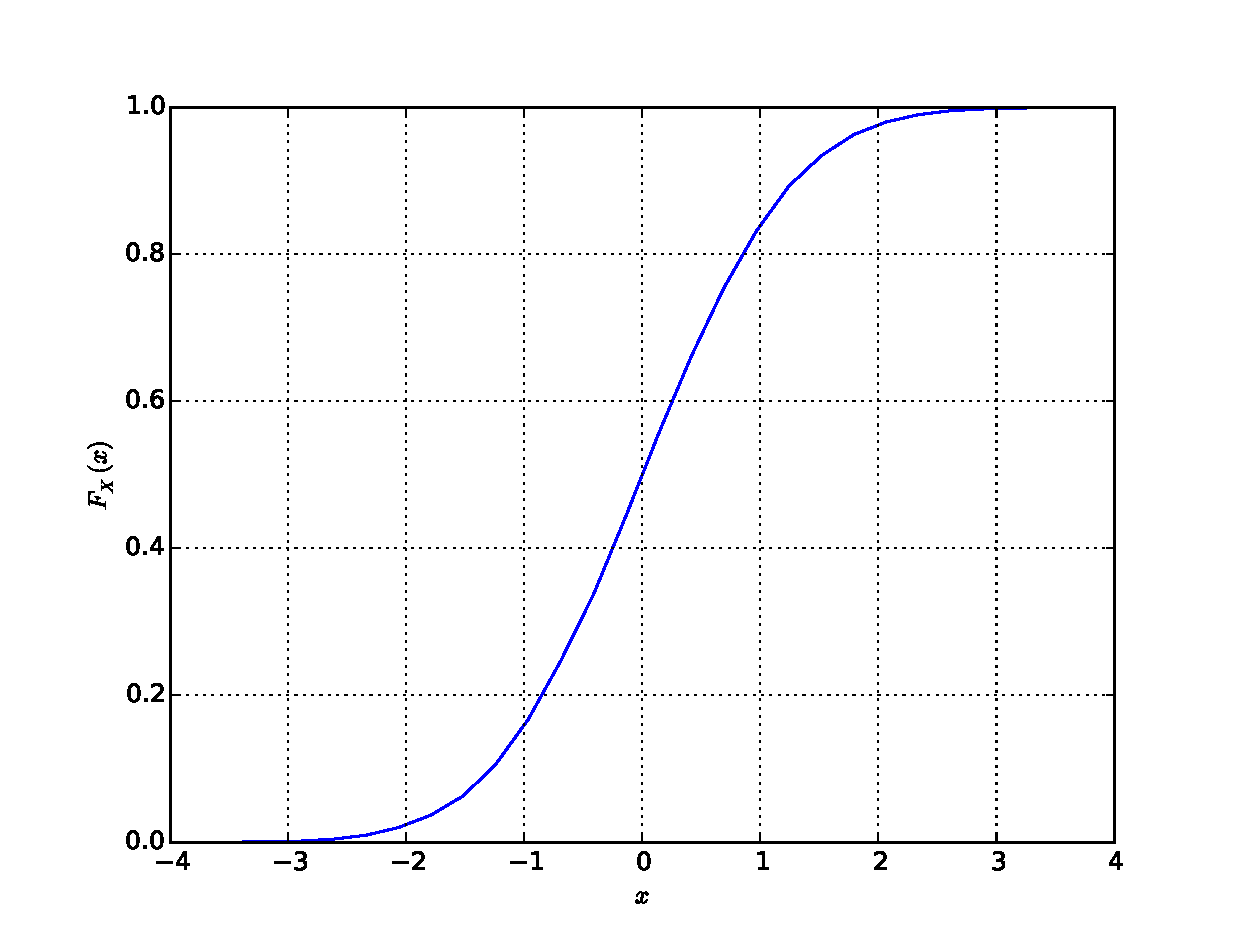
\includegraphics[width=\columnwidth]{./chapter1/figs/ch1_prob3_fig}
\caption{CDF of $X$}
\label{ch1_prob3_fig}
\end{figure}
%
\begin{problem}
List the properties of $F_X(x)$ based on Fig. \ref{ch1_prob3_fig}.
\end{problem}
%
\begin{problem}
Let
%
\begin{equation}
p_{X}(x_i) = \frac{F_{X}(x_i)-F_{X}(x_{i-1})}{h}, i = 1, 2, \dots
{h}
\end{equation}
%
for $x_i = x_{i-1}+h, x_1 = -4$. Plot $p_X(x_i)$.  On the same graph, plot
%
\begin{equation}
p_{X}(x) = \frac{1}{\sqrt{2\pi}}e^{-x^2/2}, - 4 < x < 4
\end{equation}
%
\end{problem}
%
\solution The following code yields the graph in Fig. \ref{ch1_prob4_fig}
\lstinputlisting{./chapter1/codes/1.4.py}
\begin{figure}
\centering
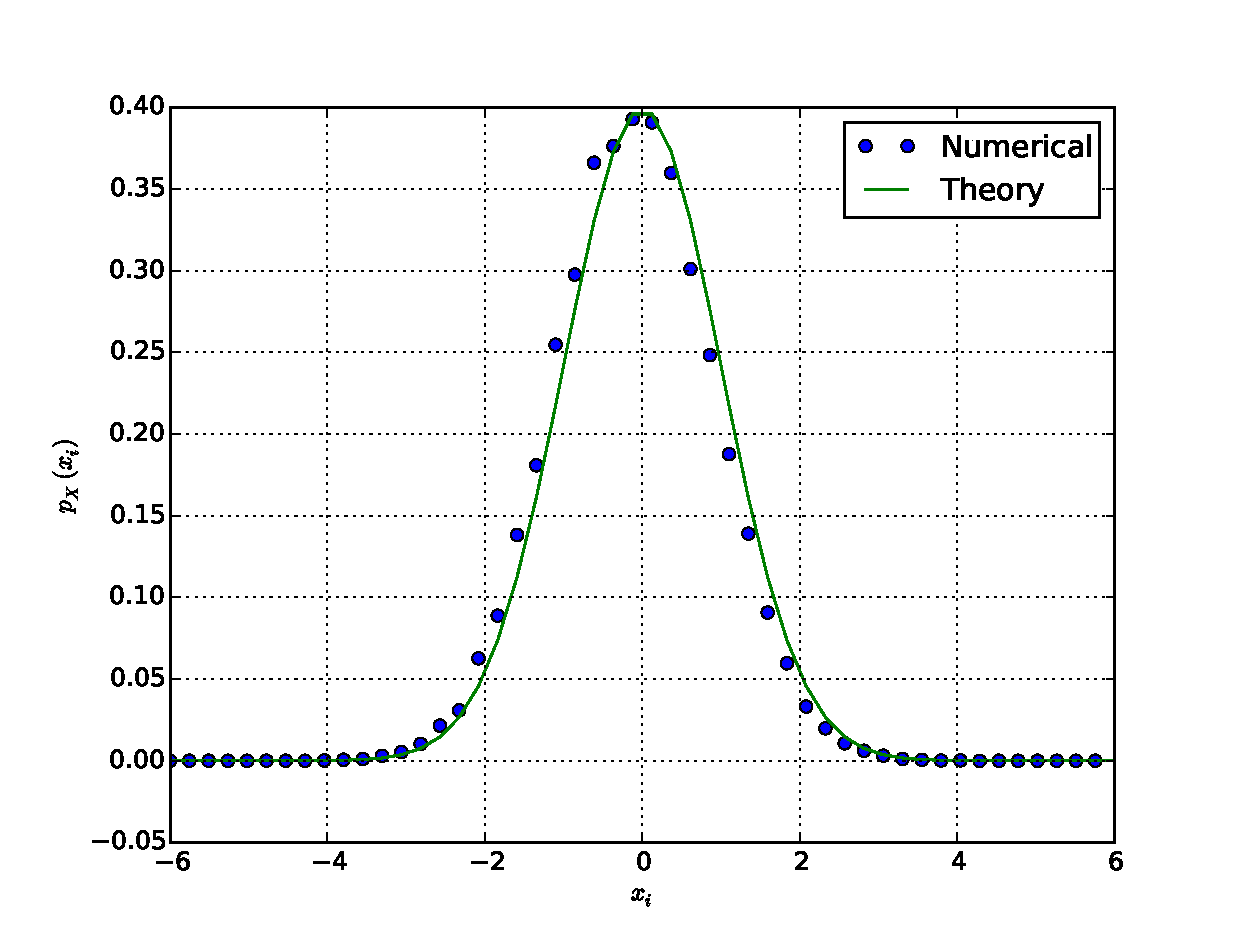
\includegraphics[width=\columnwidth]{./chapter1/figs/ch1_prob4_fig}
\caption{The PDF of $X$}
\label{ch1_prob4_fig}
\end{figure}
%
Thus, the PDF is the derivative of the CDF.  For $X\sim \mathcal{N}\brak{0,1}$, the PDF is
%
\begin{equation}
p_{X}(x) = \frac{1}{\sqrt{2\pi}}e^{-\frac{x^2}{2}}, \quad -\infty < x < \infty
\end{equation}
\begin{problem}
%
For $X\sim \mathcal{N}\brak{\mu,\sigma^2}$,
\begin{equation}
p_{X}(x) = \frac{1}{\sqrt{2\pi}\sigma}e^{-\frac{\brak{x-\mu}^2}{2\sigma^2}}, \quad -\infty < x < \infty
\end{equation}
Plot $p_{X}(x)$ for different values of $\mu$ and $\sigma$ in the same graph.  Comment.
\end{problem}







 




 





%%
%%\newpage
%\section{Hypothesis}
%%
\subsection{Detection \& Estimation}
\begin{problem}
Let $X \in \cbrak{1,-1}$.  Generate $X$ such that the numbers 1 and -1 appear with equal probability.  This is a random variable formulation of the coin tossing experiment.
\end{problem}
\solution  The following script generates the numbers 1 and -1 with 
equal probability.
\lstinputlisting{./chapter2/codes/2.1.py}
%
\begin{problem}
Verify that the script in the previous problem generates equiprobable symbols.
\end{problem}
\begin{problem}
Suppose $X \in \cbrak{1,-1}$ and 
%
\begin{equation}
Y = AX + N
\end{equation}
%
where $N \sim \gauss{0}{1}$ and $A = 4$.  Plot $Y$.
\end{problem}
\solution The following code yields Fig. \ref{ch2_bpsk_sim}
\lstinputlisting{./chapter2/codes/2.3.py}
%
\begin{figure}
\centering
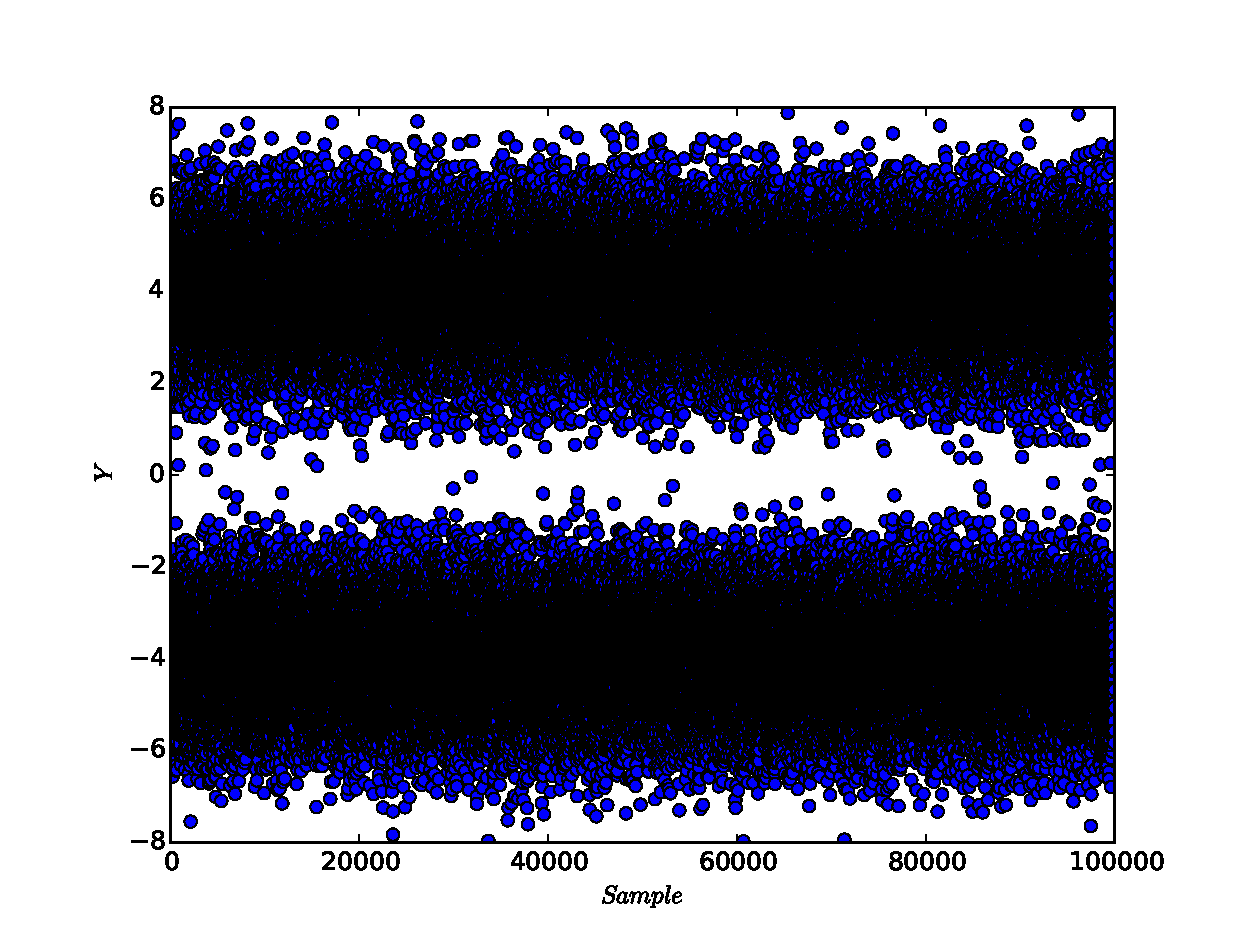
\includegraphics[width=\columnwidth]{./chapter2/figs/ch2_bpsk_sim}
\caption{Plot of $Y$}
\label{ch2_bpsk_sim}
\end{figure}
%
\begin{problem}
Given $Y$ in the previous problem, how would you decide whether $X$ is 1
or -1.
\end{problem}
%
\begin{problem}
Suppose $X=1$ and $\hat{X}$ is what you detected.  Find $\pr{\hat{X}=-1/X=1}$.
\end{problem}
%
\begin{problem}
Plot  $\pr{\hat{X}=-1/X=1}$ with respect to $A$.
\end{problem}
%
\begin{problem}
For $X \sim \mathcal{N}\brak{0,1}$, the $Q$-function is defined as
\begin{equation}
Q(x) = \pr{X > x}, \quad x > 0
\end{equation}
Express $\pr{\hat{X}=-1/X=1}$ in terms of the $Q$-function. Plot this expression with respect to $A$ and compare with the result obtained through simulation.
\end{problem}
%
\begin{problem}
The signal to noise ratio of the above system is defined as 
\begin{equation}
SNR = \frac{A^2}{\mean{N^2}}
\end{equation}
Plot the thoeretical and simulated values of $\pr{\hat{X}=-1/X=1}$ for the SNR ranging from 0 to 10 dB.
\end{problem}
%
\begin{problem}
Now consider a threshold $\lambda > 0$ and find the average probability of error. Plot this with respect to $\lambda$.
\end{problem}
%
\begin{problem}
From the graph in the previous problem, find the optimum threshold so that the probability of error is minimum.
\end{problem}
%
\subsection{The MAP criterion}
%
A Gaussian random variable $Y\sim\gauss{\mu}{\sigma^2}$ has the pdf
%
\begin{equation}
p_{Y}(x) = \frac{1}{\sqrt{2\pi}\sigma}e^{-\brak{x-\mu}^2/2\sigma^2} - \infty < x < \infty
\end{equation}
%
\begin{problem}
Plot
\begin{equation}
p_{Y}(Y|X=1) \text{ and } p_{Y}(Y|X=-1)
\end{equation}
in the same graph with respect to $A$.
\end{problem}

\begin{problem}
Graphically obtain the decision resulting from
\begin{equation}
p_{Y}(Y|X=1) \dec{1}{-1} p_{Y}(Y|X=-1)
\end{equation}
Comment.
\end{problem}

%%
%\newpage
\section{Transformation of Variables}

%\subsection{Independence}
\subsection{Using Definition}
%
\begin{problem}
Let $X_1 \sim  \gauss{0}{1}$ and $X_2 \sim  \gauss{0}{1}$. Plot the CDF and PDF of
%
\begin{equation}
V = X_1^2 + X_2^2
\end{equation}
%
\end{problem}
%
%
\begin{problem}
If
%
\begin{equation}
F_{V}(x) = 
\begin{cases}
1 - e^{-\alpha x} & x \geq 0 \\
0 & x < 0,
\end{cases}
\end{equation}
%
find $\alpha$.
\end{problem}
%
\begin{problem}
\label{ch3_raleigh_sim}
Plot the CDF and PDf of
%
\begin{equation}
A = \sqrt{V}
\end{equation}
%
\end{problem}
%
\begin{problem}
Find an expression for $F_{A}(x)$ using the definition. Plot this expression and compare with the result of problem \ref{ch3_raleigh_sim}. 
\end{problem}
%
\begin{problem}
Find an expression for $p_{A}(x)$.
\end{problem}
%
\subsection{Using Jacobian}
%
\begin{problem}
Evaluate the joint PDF of $X_1,X_2$,  given by
%
\begin{equation}
p_{X_1,X_2}(x_1,x_2) = p_{X_1}\brak{x_1}p_{X_2}\brak{x_2}
\end{equation}
%
\end{problem}
%
\begin{problem}
Let 
\begin{align}
 X_1 = \sqrt{V}\cos \theta
\\
 X_2 = \sqrt{V} \sin \theta.
\end{align}
Evaluate the Jacobian 
%
\begin{equation}
J =
\begin{vmatrix}
\frac{\partial x_1}{\partial v} & \frac{\partial x_2}{\partial v} \\
\frac{\partial x_1}{\partial \theta} & \frac{\partial x_2}{\partial \theta} 
\end{vmatrix}
\end{equation}
%
\end{problem}
%
\begin{problem}
Find
%
\begin{equation}
p_{V,\Theta}\brak{v,\theta} = \abs{J}p_{X_1,X_2}\brak{x_1,x_2}
\end{equation}
%
\end{problem}
%
\begin{problem}
Find $p_{V}(v)$.  
\end{problem}
%
%
\begin{problem}
Find $p_{\Theta}(\theta)$.  
\end{problem}
%
\begin{problem}
Are $Y$ and $\Theta$ independent?
\end{problem}
\begin{problem}
Find $p_{A}(x)$ using the Jacobian.
\end{problem}
%%
%\begin{problem}
%Let $X_1 \sim  \gauss{2}{1}$ and $X_2 \sim  \gauss{3}{1}$. Find $E\sbrak{X_1X_2}$.  Try with different mean and variances. Comment.
%\end{problem}
%

%\section{The Transform Domain}
%\begin{problem}
%Find the MGF of $X \sim \gauss{\mu}{\sigma^2}$. 
%\end{problem}
%\begin{problem}
%Find the MGF of $Y$.
%\end{problem}
%%
%\begin{problem}
%Find the PDF of $Y$ by inverting the MGF.
%\end{problem}
%%

%
\section{Conditional Probability}
%%
\begin{problem}
\label{ch4_sim}
Plot 
\begin{equation}
P_e = \pr{\hat{X} = -1|X=1}
\end{equation}
%
for 
\begin{equation}
Y = AX+N,
\end{equation}
where $A$ is Raleigh with $E\sbrak{A^2} = \gamma, N \sim \gauss{0}{1}, X \in \brak{-1,1}$ for $0 \le \gamma \le 10$ dB.
\end{problem}
%
\begin{problem}
Assuming that $N$ is a constant, find an expression for $P_e$.  Call this $P_e(N)$
\end{problem}
%
\begin{problem}
%
\label{ch4_anal}
For a function $g$,
\begin{equation}
E\sbrak{g(X)} = \int_{-\infty}^{\infty}g(x)p_{X}(x)\, dx
\end{equation}
%
Find $P_e = E\sbrak{P_e(N)}$.
\end{problem}
%
\begin{problem}
Plot $P_e$ in problems \ref{ch4_sim} and \ref{ch4_anal} on the same graph w.r.t $\gamma$.  Comment.
\end{problem}

%
\section{Two Dimensions}
%%
Let 
\begin{equation}
\mbf{y} = A\mbf{x} + \mbf{n},
\end{equation}
where 
\begin{align}
x &\in \brak{\mbf{s}_0,\mbf{s}_1}, 
\mbf{s}_0 = 
\begin{pmatrix}
1 
\\
0
\end{pmatrix},
\mbf{s}_1 = 
\begin{pmatrix}
0 
\\
1
\end{pmatrix}
\\
\mbf{n} &= 
\begin{pmatrix}
n_1
\\
n_2
\end{pmatrix},
n_1,n_2 \sim \gauss{0}{1}.
\end{align}
%
\begin{problem}
\label{ch5_fsk}
Plot 
%
\begin{equation}
\mbf{y}|\mbf{s}_0 \text{ and } \mbf{y}|\mbf{s}_1
\end{equation}
%
on the same graph using a scatter plot.
\end{problem}
%
\begin{problem}
For the above problem, find a decision rule for detecting the symbols $\mbf{s}_0 $ and $\mbf{s}_1$.
\end{problem}
%
\begin{problem}
Plot 
\begin{equation} 
P_e = \pr{\hat{\mbf{x}} = \mbf{s}_1|\mbf{x} = \mbf{s}_0}
\end{equation}
with respect to the SNR from 0 to 10 dB.
\end{problem}
%
\begin{problem}
Obtain an expression for $P_e$. Verify this by comparing the theory and simulation plots on the same graph.
\end{problem}
%

%
\section{Transform Domain}
%%
Let $X \sim \gauss{\mu}{\sigma^2}$.
\begin{problem}
Find $M_{X}\brak{s} = E\sbrak{e^{-sX}}$.
\end{problem}
%
\begin{problem}
Let 
%
\begin{equation}
N = n_1 - n_2, \quad   n_1,n_2 \sim \gauss{0}{1}.
\end{equation}
%
Find $M_{N}(s)$, assuming that $n_1$ and $n_2$ are independent.
\end{problem}
%
\begin{problem}
Show that $N$ is Gaussian. Find its mean and variance.  Comment.
\end{problem}
%

%
\section{Random Number Generation}
%%
\subsection{Uniform Random Numbers}
Let $U$ be a uniform random variable between 0 and 1.
\begin{problem}
Generate $10^6$ samples of $U$ using a C program and save into a file called uni.dat .
\end{problem}
%
\begin{problem}
Load the uni.dat file into python and plot the empirical CDF of $U$ using the samples in uni.dat.
\end{problem}
%
\begin{problem}
Verify that your CDF in the above problem is correct by plotting the theoretical $F_{U}(x)$.
\end{problem}
%
\subsection{Central Limit Theorem}
%
\begin{problem}
Generate $U_i, i = 1,2,\dots, 12$, a set of independent uniform random variables between 0 and 1 using a C program.
\end{problem}
%
\begin{problem}
Generate $10^6$ samples of the random variable
%
\begin{equation}
S = \sum_{i=1}^{12}U_i -6
\end{equation}
%
and save in a file called s.dat
\end{problem}
%
\begin{problem}
Load s.dat in python and plot the empirical PDF of $S$ using the samples in s.dat. Does it look familiar?  Comment.
\end{problem}
%
\subsection{From Uniform to Other}
%
\begin{problem}
Generate samples of 
%
\begin{equation}
V = -2\ln\brak{1-U}
\end{equation}
%
and plot its CDF.  Comment.
\end{problem}
%
\begin{problem}
Generate the Rayleigh distribution from Uniform. Verify your result through graphical plots.
\end{problem}


%\newpage
%\section{Binary Modulation}
%\input{chapter2} 
%
%\newpage
%\section{$M$-ary Modulation}
%\input{chapter3} 

%\newpage
%\section{BER in Rayleigh Flat Slowly Fading Channels}
%\input{chapter4} 

\end{document}


